\section{Quantum Radiation} \label{sec:5.1}

Until now we have considered only the total energy loss due to synchrotron radiation -- assuming implicitly that the energy loss is a continuous process. Such a view is all right for a first
 approximation since the energy loss is indeed fairly smooth on the average. But we know that all electromagnetic radiation occurs in quanta of discrete energy. And this quantization of the energy loss has significant effects on the behavior of electrons in a storage ring.\\
Each time a quantum is emitted the energy of the electron makes a small discontinuous jump. As we shall see later, the most significant quanta have energies which range from that of visible light out into soft x-rays. Although one is on shaky ground in trying to speak too quantitatively about quantum effects in a classical way, the following quasi-classical statements can be rigorously
 justified. First, the ``time'' during which a typical quantum is emitted is certainly no greater
than $\rho/\gamma c$, where $\rho$ is the radius of curvature of the trajectory and $\gamma$ is the electron energy in units of its rest energy. Since this time is much less than any other
relevant time - such as the period of a betatron or synchrotron oscillation -- we may consider-it
 to be instantaneous. Second, the emission times of the individual quanta are statistically
 independent. Since the energy change in any emission event is a very small fraction of the electron energy we may consider that the emission of successive quanta is a purely random (that is, Poisson) process.\\
The discontinuous energy change from the emission of a quantum disturbs the trajectory of the electron. The cumulative effect of many such disturbances introduces a kind of ``noise'' into the various oscillation modes causing their amplitudes to grow until the quantum excitation is, on the average, balanced by the damping of the oscillations. This process will be considered in detail for both betatron and energy oscillations in later sections.\\
A remark is perhaps required here about damping. We have, in the preceding sections, related the damping effects to radiation. You should notice that the damping depends only on the average rate of emission of energy and not on any of its other statistical properties. So when considering quantum effects we may take the same damping we have already found -- understanding
 that it is due to the average rate of energy loss in all quantum energies. The excitation
 effects will be due to the fluctuations in the radiation about its average rate (One could, of
course, treat both the average and fluctuation effects together, but to do so would only add unwarranted complications).\\
In considering the effects of radiation fluctuations on the oscillations of an electron in a storage ring we shall need to know certain properties of the quantized radiation. I wish now to look at these properties.\\
From the classical view, the synchrotron radiation is emitted with a continuous spectrum of frequencies. (The frequency spectrum was first calculated by \cite{13} Schwinger, a derivation
 is also given in Jackson \cite{10}.) Consider the radiation emitted by an electron in some finite time interval $\Delta t$. Suppose we examine the radiation field which corresponds
 -- by a suitable time retardation -- to the emission in $\Delta t$, and for each direction in space, make a Fourier analysis of the radiation field. The frequency spectrum will, in general,
 be different for each direction. But we may average the spectrum over all directions to define a radiated power spectrum $\mathscr{P}(\omega)$ such that $\mathscr{P}(\omega)d\omega \Delta t$ is the energy radiated in $\Delta t$ with angular frequencies between $\omega$ and $\omega + d\omega$. Clearly, the definition makes sense only if $\Delta t$ is sufficiently large that most of the energy is found in frequencies greater than $1/\Delta t$. Recall now, that the radiation
 is typically emitted within the angle $1/\gamma$ of the electron's velocity vector. Such an angle is swept out in the time $\rho/\gamma c$, where $\rho$ is the local radius of curvature
 of the trajectory. So a time interval $\approx \rho/\gamma c$ should contain most of the impulse of radiation; and it should, therefore, represent a suitable magnitude for $\Delta t$. We shall see later that it is indeed so.\\
With the definition given for $\mathscr{P}(\omega)$ we may permit it to be a slowly varying
function of time and we shall not be in any difficulty provided only that $\mathscr{P}(\omega)$
 (and therefore, $\rho$ or $\gamma$ on which it depends) does not change appreciably in $\Delta t$. This condition is generally satisfied\footnote{The important results of this part actually require only that $\rho$ and $\gamma$ do not change appreciably in a time $\rho/\gamma c$ which is much smaller than $\Delta t$.} for storage rings, so we may consider that $\mathscr{P}(\omega)$ is an ``instantaneous'' power spectrum whose integral over $\omega$ is the instantaneous radiated power defined earlier,
\begin{align}
	P_\gamma = \int_0^{\infty} \mathscr{P}(\omega) d\omega.
\end{align}
The power spectrum can be written in the convenient form:
\begin{align} \label{eq:5.2}
	\mathscr{P}(\omega) = \dfrac{P_\gamma}{\omega_c} S\left( \dfrac{\omega}{\omega_c} \right),
\end{align}
with $\omega_c$ a constant defined by
\begin{align}
	\omega_c = \dfrac{3}{2} \dfrac{c \gamma^3}{\rho}.
\end{align}
The number $\omega_c$ is called the critical frequency\footnote{Caution!
 Some writers,for example Jackson, define the critical frequency with a different numerical factor.}, notice that it is approximately equal to $\gamma^3$ times the angular revolution
 frequency of the electron. The spectral function $S(\omega/\omega_c)$ is a pure algebraic
 function of its argument which can be expressed by
\begin{align}
	S(\xi) = \dfrac{9 \sqrt{3}}{8\pi} \xi \int_\xi^{\infty} K_{5/3} (\bar{\xi}) d\bar{\xi}.
\end{align}
where $K_{5/3}$ is the modified Bessel function of the second kind. It follows from the definition of Eq.~\eqref{eq:5.2} that $S$ is normalized so that
\begin{align}
	\int_0^{\infty} S(\xi) d\xi = 1.
\end{align}
The form of the spectral function is shown in Fig.~\ref{fig:fig42}. Its behavior for large and for small arguments -- which can easily be obtained from the asymptotic
\begin{figure}[!htb]
	\centering
	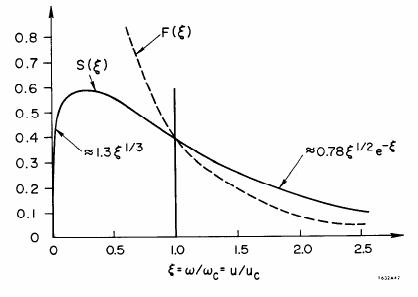
\includegraphics[width=0.8\linewidth]{./Figuras/fig42.jpeg}
	\caption{Normalized power spectrum $S$ and photon number spectrum $F$ of synchrotron radiation.}
	\label{fig:fig42}
\end{figure}
behavior of the Bessel function -- is sometimes useful.
\begin{align} \label{eq:5.6}
	\text{For }\xi << 1; \hspace{5mm} & S(\xi) \approx \dfrac{9}{2\sqrt[3]{2}\Gamma(1/3)} \xi^{1/3}, \\
    \text{For }\xi >> 1; \hspace{5mm} & S(\xi) \approx \dfrac{9\sqrt{3}}{8 \sqrt{2\pi}} \xi^{1/2} e^{-\xi},
\end{align}
 where $\Gamma$ is the Gamma function. The power spectrum $\mathscr{P}(\omega)$ is obtained from $S(\xi)$ by Eq.~\eqref{eq:5.2}. Don't forget that both $P_\gamma$ -- see Eq.~\eqref{eq:4.4} -- and $\omega_c$ depend on both $\gamma$ and $\rho$. It is clear from Fig.~\ref{fig:fig42} that most of the power is found in frequencies near $\omega_c$ (since $\omega_c$ is $\gamma^2$ larger
 than the inverse of the $\Delta t$ defined earlier, the assumptions made there are now justified).\\
You know that electromagnetic radiation at the angular frequency $\omega$ is emitted in quanta of energy $u = \hslash \omega$ , where $\hslash$ is Plank's constant reduced by $2\pi$ ($\hslash = h/2\pi = 6.58 \times 10^{-16}$eV-sec). Let $n(u)du$ be the number of quanta emitted per unit time with energies between $u$ and $u + du$. The power emitted in these quanta is $un(u)du$,
which must be the same as the power emitted in the frequency interval $d\omega = du/\hslash$
at the frequency $\omega = u/\hslash$; namely,
\begin{align}
	u n(u) du = \mathscr{P}(u/\hslash)du/\hslash.
\end{align}
Taking $\mathscr{P}(\omega)$ from Eq.~\eqref{eq:5.2} the quantum distribution function can be written as
\begin{align}
	n(u) = \dfrac{P_\gamma}{u_c^2} F\left( \dfrac{u}{u_c} \right),
\end{align}
with
\begin{align} \label{eq:5.9}
	u_c = \hslash \omega_c = \dfrac{3}{2} \dfrac{\hslash c \gamma^3}{\rho},\\
    F(\xi) = \dfrac{1}{\xi}S(\xi).
\end{align}
Like the frequency spectrum, the quantum spectrum is, apart from the scale factor $P_\gamma/u_c^2$ a universal function of the ratio $u/u_c$.
The function $F(\xi)$ is also shown in Fig.~\ref{fig:fig42}. The rate of emission of quanta per unit energy interval diverges at low energies\footnote{The spectrum is, anyway, questionable for $u < u_c/\gamma^3 \approx \hbar c/\rho$, according to the conditions mentioned earlier.}. But only as $u^{-2/3}$, so the rate of emission of the quanta in any finite interval of quantum energies -- an integral
 over $u$ -- is finite.\\
Let's let $\mathscr{N}$ stand for the total rate of emission of quanta (of all energies):
\begin{align}
	\mathscr{N} = \int_0^\infty n(u) du.
\end{align}
From the asymptotic expressions for $S(\xi)$ in \eqref{eq:5.6}, its complete integral
 is clearly $\approx 1$. It is actually $\dfrac{15\sqrt{3}}{8}$ so
\begin{align} \label{eq:5.12}
	\mathscr{N} = \dfrac{15\sqrt{3}}{8} \dfrac{P_\gamma}{u_c}.
\end{align}
The mean quantum energy would be defined:
\begin{align}
	\mean{u} = \dfrac{1}{\mathscr{N}} \int_0^\infty u n(u) du.
\end{align}
The integral is just $P_\gamma$ so the mean quantum energy is
\begin{align}
	\mean{u} = \dfrac{8}{15\sqrt{3}} u_c = (0.32...) u_c.
\end{align}
Speaking roughly, we may say that the radiation is emitted in quanta of a typical energy about $u_c$, and at a mean rate of about $P_\gamma/u_c$. For a 1 GeV electron moving on a 5 meter radius trajectory,
\begin{align*}
	P_\gamma &= 1.7 \times 10^{11}\, \text{eV}\,\text{sec}^{-1},\\
    u_c &= 437\, \text{eV},\\
    \mathscr{N} &= 3.2 P_\gamma / u_c = 1.3 \times 10^9\, \text{sec}^{-1}.
\end{align*}
It is amusing to notice that the mean number of quanta emitted per radian of trajectory depends only on the electron energy. It is, in fact, very nearly equal to simply the product of $\gamma$ and the fine structure constant:
\begin{align}
	\text{(Mean number of quanta per radian)} = \dfrac{5}{2\sqrt{3}} \dfrac{\gamma}{137}.
\end{align}
For a 1 GeV electron, the number is about 20. The actual number in any time interval fluctuates
 as the Poisson distribution corresponding to the mean number. It is then understandable
 that with such small numbers the fluctuations may be significant.\\
 We shall see later that the quantum excitation of electron oscillations in a storage ring depends not only on the mean rate of quantum emission, but also on the mean-square quantum energy. We would expect $\mean{u^2}$ to be about equal to $u_c^2$; as indeed it is.
 If you work it out in detail you will find that
\begin{align}
	\mean{u^2} = \dfrac{11}{27} u_c^2.
\end{align}
The quantity that will enter in the quantum excitation of oscillations is in fact, the product of the mean square quantum energy with the mean rate; namely
\begin{align} \label{eq:5.17}
	\mathscr{N} \mean{u^2} = \int_0^\infty u^2 n(u) du.
\end{align}
It will be convenient to write, using Eq.~\eqref{eq:5.12}
\begin{align} \label{eq:5.18}
	\mathscr{N} \mean{u^2} = C_u u_c P_\gamma,
\end{align}
with
\begin{align}
	C_u = \dfrac{55}{24\sqrt{3}} = 1.32...
\end{align}
It is important to keep in mind that both $u_c$ and $P_\gamma$ are functions of the electron
energy and of the local radius of curvature $\rho$ of the trajectory. Taking $u_c$ from Eq.~\eqref{eq:5.9} and $P_\gamma$ from Eq.~\eqref{eq:4.4},
\begin{align}
	\mathscr{N} \mean{u^2} = \dfrac{3 C_u C_\gamma}{4 \pi} \dfrac{\hslash c^2}{(mc^2)^3} \dfrac{E^7}{\rho^3} = \dfrac{55}{24\sqrt{3}} r_e \hslash mc^4 \dfrac{\gamma^7}{\rho^3}
\end{align}
At a fixed radius the quantum excitation varies as the seventh power of the energy!
